% Created 2012-11-28 Wed 17:52
\documentclass[bigger]{beamer}
\usepackage[utf8]{inputenc}
\usepackage[T1]{fontenc}
\usepackage{fixltx2e}
\usepackage{graphicx}
\usepackage{longtable}
\usepackage{float}
\usepackage{wrapfig}
\usepackage{soul}
\usepackage{textcomp}
\usepackage{marvosym}
\usepackage{wasysym}
\usepackage{latexsym}
\usepackage{amssymb}
\usepackage{hyperref}
\tolerance=1000
\titlegraphic{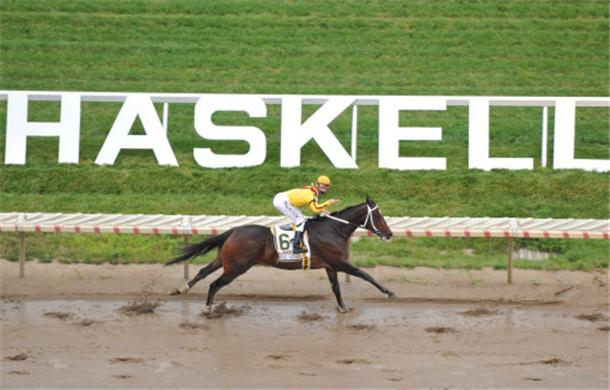
\includegraphics{../pictures/haskell_horse.jpg}}
\setbeamertemplate{navigation symbols}{}
\mode<beamer>{\usetheme{CambridgeUS}}
\institute[GWU]{The George Washington University}
\usepackage{listings}
\lstset{language=Haskell, basicstyle=\scriptsize}
\providecommand{\alert}[1]{\textbf{#1}}

\title{30\% Demonstration}
\author{Andrew Hirsch}
\date{\today}
\hypersetup{
  pdfkeywords={},
  pdfsubject={},
  pdfcreator={Emacs Org-mode version 7.8.11}}

\begin{document}

\maketitle


\begin{frame}[fragile]
\frametitle{The Form of Data}
\label{sec-1}


\begin{itemize}
\item Datatypes: ``Sum'' of constructors
\item Constructors: functions $F$ that take data of type a into data $F a$
\end{itemize}

\begin{lstlisting}
data Directions = North Int
                | South Int
                | East Int
                | West Int
\end{lstlisting}

\begin{lstlisting}
data Directions' = North' :+: South' :+: East' :+: West'
data North' = North' Int
data South' = South' Int
data East'  = East' Int
data West'  = West' Int
\end{lstlisting}

$$\mathtt{Directions} \cong \mathtt{Directions'}$$
\end{frame}
\begin{frame}[fragile]
\frametitle{The Form of Data, Ctd.}
\label{sec-2}


\begin{itemize}
\item What about recursive data types?
\end{itemize}

\begin{lstlisting}
data ListInt = Nil
             | Cons Int ListInt
\end{lstlisting}

\begin{lstlisting}
data ListInt' = Nil :+: Cons
data Nil e = Nil
data Cons e = Cons Int e
\end{lstlisting}

\begin{itemize}
\item What's special about \verb~Cons~?
\begin{itemize}
\item Cons is a \emph{functor}
\item Cons should have a function \lstinline{fmap :: (a -> b) -> (Cons a -> Cons b)}
\item Nil is also a functor, trivially
\item ListInt' is also a functor
\end{itemize}
\end{itemize}

$$\mathtt{ListInt} \cong \mathtt{ListInt'}?$$
\end{frame}
\begin{frame}[fragile]
\frametitle{Tying the Recursive knot}
\label{sec-3}


\begin{lstlisting}
data Term f = f (Term f)
\end{lstlisting}

\begin{itemize}
\item $\mathtt{ListInt} \cong \mathtt{Term (ListInt')}$
\item ``Tying the Recursive Knot''
\end{itemize}
\end{frame}
\begin{frame}[fragile]
\frametitle{Parsing into Tied Structures}
\label{sec-4}


\begin{lstlisting}

parseListInt :: Parser ListInt'
parseListInt = parseCons <|> parseNil

parseCons :: Parser ListInt'
parseCons = do
  i <- parseInt
  char ':'
  l <- parseListInt
  return $ iCons i l

parseNil :: Parser ListInt'
parseNil = do
  string "[]"
  return iNil

\end{lstlisting}
\end{frame}
\begin{frame}[fragile]
\frametitle{Parsing into Untied Structures}
\label{sec-5}


\begin{lstlisting}

parseListInt :: Parser e -> Parser (ListInt' e)
parseListInt p = (do
                    c <- parseCons e
                    return $ inr c)
             <|> (do
                    n <- parseNil e
                    return $ inl c)

parseCons :: Parser e -> Parser (Cons e)
parseCons p = do
  i <- parseInt
  char ':'
  e <- p
  return $ Cons i p

parseNil :: Parser e -> Parser (Nil e)
parseNil p = do
  string "[]"
  return Nil

\end{lstlisting}
\end{frame}
\begin{frame}[fragile]
\frametitle{Tying while parsing?}
\label{sec-6}


\begin{itemize}
\item Can we use the code last slide to get a parser for \verb~Term(ListInt')~?
\item Need some sort of \emph{fixed point} for parsers
\item None currently exists
\end{itemize}
\end{frame}
\begin{frame}
\frametitle{Solution: Side Step}
\label{sec-7}


\begin{itemize}
\item We instead introduce grammars with inheritance
\item Grammars can \emph{extend} other grammars
\item Those then get translated into a full grammar
\item Grammars have ADTs and Happy files generated automatically
\item Happy = YACC for Haskell
\end{itemize}
\end{frame}
\begin{frame}[fragile]
\frametitle{Example: EBNF for EBNF}
\label{sec-8}


\scriptsize

\begin{verbatim}
Grammar EBNF {

EBNF ::= {Production}

Production ::= Identifier "::=" Expression ".".

Expression ::= Term {"|" Term}.

Term ::= Factor {Factor}.

Factor ::= Identifier
         | "[" Expression "]"
         | "(" Expression ")"
         | "{" Expression "}"
         | Literal.

Identifier ::= Character { Character }.

Literal ::= "'" Character { Character }
          | '"' Character { Character }.
 
}

\end{verbatim}
\end{frame}
\begin{frame}[fragile]
\frametitle{Example: EBNF Subgrammar for EBNF Subgrammars}
\label{sec-9}


\scriptsize

\begin{verbatim}

Grammar EBNFSubgrammar extends EBNF {

Production ::+ Identifier "::+" Expression.

}

\end{verbatim}
\end{frame}

\end{document}
